\documentclass{article}
\usepackage{graphicx}
\usepackage[a4paper, total={6in, 8in}]{geometry}
\usepackage{booktabs}
\usepackage{siunitx}
\sisetup{
    detect-all,
    table-number-alignment = center,
    table-figures-integer = 3,
    table-figures-decimal = 4,
    table-figures-exponent = 2,
    exponent-product = \times,
    output-exponent-marker = e
}
\usepackage{caption}
\captionsetup[table]{skip=5pt}
\usepackage{url}

\title{A log-link negative binomial-error GLM model to predict \textit{E. nigrita} abundance}
\author{Oliver Ekström Todreas \\ BIOS15}
\date{30 November 2025}

\begin{document}

\maketitle
\thispagestyle{empty}
\newpage

\section{Introduction}

The importance of conserving species should not be understated. However, the process of maintaining records on species in all corners of the world is likely one that could benefit from optimization. In particular, models that predict how species  abundance changes using readily available climate data have the potential to allow researchers to monitor species abundance and catch warning signs before going into the field.

In this paper, we propose a generalized linear model (GLM) that predicts the abundance of the bee species \textit{Eulaema nigrita} in the Brazilian Atlantic forest using data from the \textit{Worldclim} dataset. Furthermore, we take into account the number of hours spent sampling to ensure that our model controls for varying degrees of sampling effort.

\section{Methods}

To accurately assess \textit{E. nigrita} abundance, multiple testing steps were taken to ensure that we produced a strong model. First, we fitted three different linear models, two of them GLMs with log link functions, to the data and examined their performance relative to each other. The first simple multiple linear regression model was defined as

$$
Y = \beta_0 + \beta_1 X_1 + \beta_2 X_2 + \beta_3 X_3 + \beta_4 X_4 + \epsilon
$$

Where $Y$ is the predicted abundance of \textit{E. nigrita}, $\beta$ are the model coefficients, $X$ are the predictor values, and $\epsilon$ accounts for the differences between the predicted and the true abundance of \textit{E. nigrita}. The predictor variables $X_1$ through $X_4$ are sampling effort in logarithmic hours, mean annual percipitation (MAP) in mm, the temperature seasonality (Tseason) given as 100 times the standard deviation of the monthly temperature in °C, and the percipitation seasonality (Pseason) given as the unitless coefficient of variation of monthly percipitation. The latter three predictors are all \textit{Worldclim} data.

Considering that the response variable \textit{E. nigrita} abundance is structured as count data, we identified the risk that residuals may not have been normally distributed had we used a linear model without a link function. To test this, we fitted a linear model without a link function and visually examined the distribution of the residuals and the QQ plot of the residuals. Following these observations, we focused on the two remaining GLMs, defined as

$$
\eta = \beta_0 + \beta_1 X_1 + \beta_2 X_2 + \beta_3 X_3 + \beta_4 X_4 + \epsilon
$$

Where $\eta$ is the predicted output on the link scale. We identified the natural log as an appropriate link function $g$, defined as

$$
g = ln(x)
$$

Whose inverse back-transforms predicted outputs on the link scale $\eta$ into predicted outputs on the data scale $Y$ such that

$$
Y = g^{-1}(\eta)
$$

The two remaining GLMs differed in their error distributions, the former with Poisson errors and the latter with negative binomial errors. To select the optimal model, overdispersion and Akaike information criteria (AIC) were assessed. First, overdispersion in the data was quantified as the ratio of residual deviance to the residual degrees of freedom in the Poisson-error model. The ratio's large value suggested that the count data's variance increased disproportionately compared to the mean. Before ultimately selecting the negative binomial-error model, the AIC's of both models were compared.

Finally, we assessed whether to drop any of our predictor variables. We found that MAT (mean annual temperature (°C$\times 10$), not discussed above to avoid confusion) had a far less significant impact on the model than the other predictors, leading us to drop the predictor. Following that, we performed a multicollinearity check to ensure that we would drop any highly correlated variables.

\section{Results}

We found that each predictor variable had a significant effect on \textit{E. nigrita} abundance. Generally, holding other variables constant, sampling effort and Pseason were positively correlated with \textit{E. nigrita} abundance (Figure 1A, 1D), while MAP and Tseason were negatively correlated with \textit{E. nigrita} abundance (Figure 1B, 1C).

\begin{figure}[htp]
    \centering
    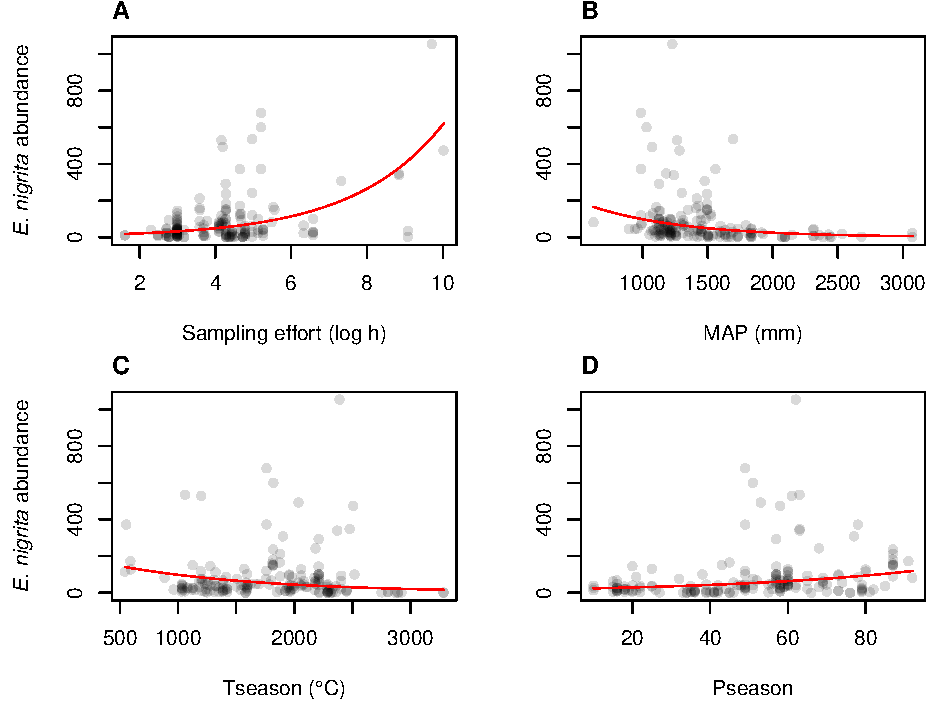
\includegraphics[width=12cm]{fig1.pdf}
    \caption{\textit{E. nigrita} abundance was positively correlated with sampling effort (A) and Pseason (D), while it was negatively correlated with MAP (B) and Tseason (C), while all other variables were held constant. The linear model is shown in red. For a given plot, the predicted \textit{E. nigrita} abundance was a function of the plotted variable, while the other variables in the model were held constant at their means.}
    \label{fig:galaxy}
\end{figure}

A 1 mm increase in MAP corresponded with a decrease of 0.999 in expected \textit{E. nigrita} abundance. A 1 °C change in Tseason corresponded with a decrease of a factor of 0.999 in response, while a change of one in Pseason corresponded with an increase of a factor of 1.02 in the response. The largest change in response following a one-unit change in predictor came from sampling effort. A change in 1 log hour of sampling effort corresponded with an increase of a factor of 1.52 in the response (Table 1).

\begin{table}[h!]
\centering
\captionsetup{skip=10pt}
\caption{Back-transformed estimates from model.}

\begin{tabular}{
    l
    S[table-format=3.3]     % Backtransformed estimate
    S[table-format=1.5]     % Std. Error
    S[table-format=-2.2]    % z value
    S[scientific-notation=true, table-format=1.2e2] % p-value
}
\toprule
{Variable} & {$e$-exponentiated estimate} & {Std.~error} & {$z$-value} & {$p$-value} \\
\midrule
Intercept               & 103     & 0.432    & 10.7   & 6.39e-27 \\
Sampling effort (log h)& 1.52    & 0.0575   & 7.33   & 2.28e-13 \\
MAP (mm)       & 0.999   & 0.000199 & -6.91  & 4.73e-12 \\
Tseason (°C)   & 0.999   & 0.000154 & -5.14  & 2.68e-07 \\
Pseason                 & 1.02    & 0.00367  & 5.34   & 9.35e-08 \\
\bottomrule
\end{tabular}

\end{table}

Deviances in the model were 361.71 and 206.01 for the null deviance and residual deviance respectively, and there were 177 and 173 degrees of freedom respectively. AIC was 1783.4 (Table 2).

\begin{table}[h!]
\centering
\caption{Model deviance and AIC.}

\begin{tabular}{l S[table-format=3.2] S[table-format=3.0]}
\toprule
Statistic & {Value} & {Degrees of freedom} \\
\midrule
Null deviance      & 361.71 & 177 \\
Residual deviance  & 206.01 & 173 \\
AIC                & 1783.4 & {} \\
\bottomrule
\end{tabular}

\end{table}

\section{Discussion and Conclusion}

In this paper we propose a GLM with negative binomial errors to explain \textit{E. nigrita} abundance with readily available climate data from the \textit{Worldclim} dataset. We found that all the included predictors had a significant effect on the response variable when other predictors were held constant.

It is noteworthy that the predictors MAP and Pseason had opposite effects on predicted \textit{E. nigrita} abundance given that both are measures of percipitation. This could be due to a host of reasons. For one, it is possible that percipitation favors \textit{E. nigrita} abundance at certain points in the year, while rain at other points in the year have no effect. One could also imagine a year where the rain over the entire year (MAP) was low due to extensive droughts, which had the effect of producing sporadic heavy rainfall, causing the percipitation seasonality (Pseason) to be high. In this low MAP, high Pseason year, it might be expected that \textit{E. nigrita} flourish.

Furthermore, our aim to find a model that accounted for sampling effort proved fruitful, since we found that sampling effort had the largest effect on \textit{E. nigrita} abundance per predictor unit change. The dataset analyzed included quite few surveys conducted with a sampling effort greater than 6 log hours. Nonetheless, it is above this threshold where \textit{E. nigrita} abundance appears to increase drastically (Figure 1A). Perhaps if a similar survey were to be repeated with greater sampling effort per sample, higher \textit{E. nigrita} counts may be observed. If this trend holds, there may be reason to believe that there are flourishing \textit{E. nigrita} communities that are not easily surveyed.

\section{Appendix}

The data, code, and figures used to produce this report can be downloaded at the link below:
\url{https://github.com/otodreas/BIOS15_Report-2}.

\end{document}
